% Metódy inžinierskej práce

\documentclass[10pt,a4paper,column]{article}
\usepackage[top=4cm, bottom=4cm, left=3cm, right=3cm, marginparwidth=1.75cm]{geometry}
\usepackage[english]{babel}
\usepackage[labelfont=bf]{caption}
\usepackage[T1]{fontenc}
\usepackage[IL2]{fontenc} 
\usepackage[utf8]{inputenc}
\usepackage{graphicx, subcaption, multicol}
\usepackage{url} % príkaz \url na formátovanie URL
\usepackage{hyperref} % odkazy v texte budú aktívne (pri niektorých triedach dokumentov spôsobuje posun textu)

\usepackage{cite}
%\usepackage{times}

\pagestyle{headings}

\title{Browser fingerprint and privacy issues regarding data collection from search engines\thanks{Semestrálny projekt v predmete Metódy inžinierskej práce, ak. rok 2023/24, vedenie: Ing. Mohammad Yusuf Momand, MSc.}} % meno a priezvisko vyučujúceho na cvičeniach

\author{Viktória Latičová\\[2pt]
	{\small Slovenská technická univerzita v Bratislave}\\
	{\small Fakulta informatiky a informačných technológií}\\
	{\small \texttt{xlaticova@stuba.sk}}
	}

\date{\small 12. december 2023} % upravte



\begin{document}
\maketitle

\begin{abstract}
This article aims to reflect on some key privacy concerns caused by search engines collecting data while searching on the internet. Besides the obvious task of searching by keywords, they also collect user data
to create detailed profiles. Browser fingerprinting techniques identify users uniquely, allowing cross-site tracking leading to location tracking, privacy invasion, or third-party sharing. Protecting users' privacy requires not only technological solutions- because completely removing our browser fingerprint would make searching impossible, but also legal regulations and raising public awareness and education about this topic.
\end{abstract}


\section{Introduction}
Tracking users across various websites is not a novel concept in the online realm. Websites often monitor users without their awareness, and these practices can serve various purposes. Some are well-intentioned, such as personalization and user interface optimization, while others involve the sale of user information to third-party websites or the more extensive tracking of personal data.
\section{browser fingerprint} 

The most well-known tracking technique to the public is collecting cookies, which are then stored on users' devices for later use\cite{Fpstalker}. But unlike cookies, creating a browser fingerprint actually does not require the permission of the user and as it is not stored in any device, it does not leave a trace either. Tracking via cookies also became harder as modern browser extensions automatically delete them after a certain time.

A browser fingerprint is essentially a user profile created from data collected during online activities\cite{FingerprintDefender}. This profile includes a wide range of device-related information, such as IP address, time zone, CPU details, screen resolution, plugins, ad-blockers, and much more. Some webmail services are even recognized for inspecting emails of users, who have never granted permission to them.\cite{webtrackingMID} Their unique fingerprint is now a new tool for websites to assign their identity to activities on the internet.

\begin{figure}
    \centering
    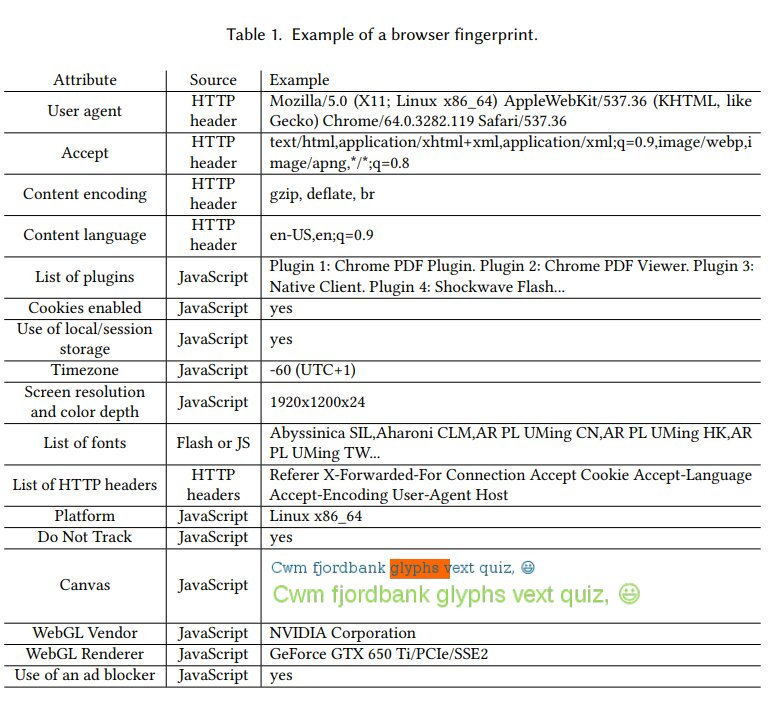
\includegraphics[scale = 0.4]{Browser-Fingerprint-example.jpg}
    \caption{Example of a browser fingerprint. \cite{table}(Laperdrix et al., 2019)}
    \label{fig:1}
\end{figure}


\subsection{click tracking} 
One of the first methods, but still used for obtaining information from users is quite straightforward – using URLs\cite{webtrackingMID}. Many people remain unaware that major search engines like Google, Yahoo, or Bing permit this kind of click tracking\cite{hostFingerprint}. Tracking clicks on links is not always employed for bad purposes. In most cases, it is used in affiliate marketing by companies for statistical and analytical purposes, and to better understand the user's behavior.

In certain cases, attackers can create a unique link that initially redirects the user to a different site, takes information that is needed, and swiftly redirects the user to the destination site. This method can be dangerous because of its almost non-existent chance of being discovered just by looking at the URL. 

\subsection{geolocation fingerprinting}

One of the most straightforward features to identify is the IP address of a user, However, obtaining a user's location from an IP is a more complicated process, known as geolocation. When a user accesses a website, their IP address is captured. IP geolocation databases of providers can provide an approximate geographic location. This information can include the country, city, or even latitude and longitude. The presence of a proxy can be easily detected and, with some skill, even bypassed\cite{webtrackingMID}.

At the same time, it is important to note that geolocation is not always 100\% accurate. It only provides an approximation of location. Also, a VPN or a Tor (The Onion Router) can be used to mask the real IP address.

\subsection{operating system fingerprinting}
Operating system fingerprinting is a technique used for detecting the operating system running on a remote device when connected to a network. Based on an article\cite{OSfingvANTA} of Aksoy et al. OS detection helps improve network management, ensures that the software is compatible with the user's operating system, and also can detect unauthorized attacks. Javascript and Flash have the ability to detect information about operating systems of devices\cite{webtrackingMID}. Information like local timezone is detectable in a blink of an eye. According to Bujlow et al.\cite{webtrackingMID}, Flash has the ability to detect various system features, such as audio capabilities, camera and microphone access permissions, and printing support.

We can categorize OS fingerprinting into two types:\cite{OSfingerprinting}

passive fingerprinting, where the attacker does not send out any packets to the victims. In this method, the attacker does not directly communicate with the target system but rather waits for the target to establish a connection, most of the time by being tricked to connect.

Active fingerprinting, on the other hand, requires the attacker to send specific network requests to the victim in order to be able to determine system information.

In summary, passive fingerprinting relies on the victim's system making the first move, while active fingerprinting requires the attacker to actively send requests to the victim's system to discover its operating system.
 

\subsection{browser extensions fingerprinting}
Browser extensions are programs, that are written to add functionalities to the browser. They offer users the ability to block ads, take screenshots, manage passwords, or assist when researching on the internet\cite{carnus}. using more extensions extends the tracking powers of attacker, as users become more and more unique for fingerprinting. Some extensions, without the knowledge of the user, can be also designed to collect data from the user from the start\cite{bfautt}. These extensions are written using HTML, CSS, and JavaScript, which gives them the capability to track user activity similarly to websites\cite{FingerprintDefender}. The research of Oleksii Starov and Nick Nikiforakis\cite{Starov:powers} from the year 2017 identified that: „6.3\% of popular Google Chrome extensions leak privacy-sensitive information to at least one-third party“. 

\begin{figure}
    \centering
    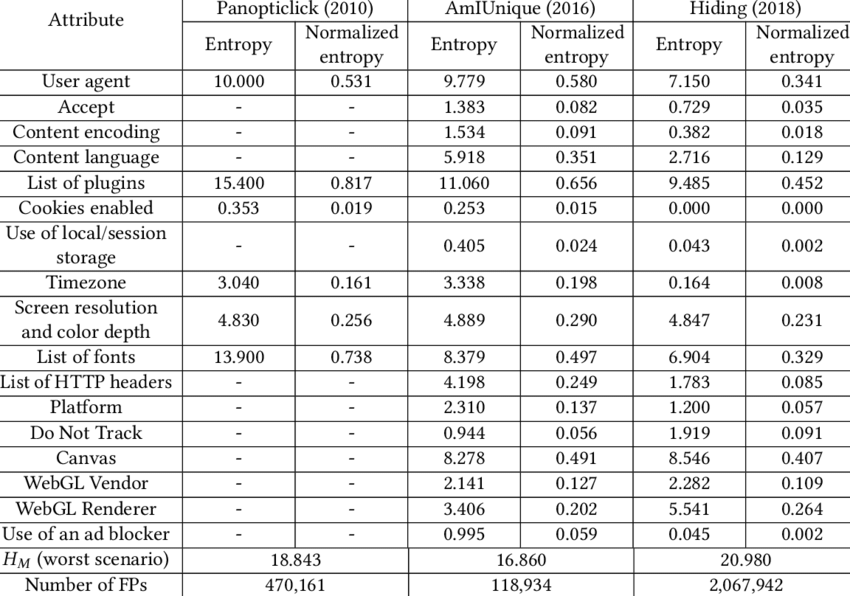
\includegraphics[scale = 0.4]{Entropy.png}
    \caption{Browser attributes, their entropy and their normalized entropy \cite{table}(Laperdrix et al., 2019)}
    \label{fig:2}
\end{figure}                                                                                

As we can see in Figure \ref{fig:2} provided by the Panopticlick\cite{panopticlick}, AmIUnique\cite{amiunique}, and Hiding in the Crowd\cite{hiding} studies, the biggest entropy in browser fingerprints is created by the selection of browser, the number of plugins that the user uses when searching, and also the list of fonts used by the device. A non-negligible part is also made of the language used by the user or the screen resolution of the device.

\section{security risks}
With fingerprinting, attackers can find weaknesses in a user's device or browser, which could result in targeted attacks. Users can be uniquely identified and tracked via their browser fingerprints, even if they use private browsing modes or get rid of their cookies. It might be challenging for users to stay anonymous online after being exposed to profiles created with browser fingerprinting. To reduce the uniqueness of their fingerprint, some users may disable or alter browser security measures\cite{webtrackingMID}, which then compromise their online security.
\section{potential solutions}
The easiest way to decrease the uniqueness of our browser fingerprint is by using multiple search engines for different tasks. Doing this makes it a lot harder for attacker to link the user's activity to everything they search. On the other hand, this approach decreases user experience when searching.

As the highest entropy of browser fingerprint is created when using plugins and extensions, in theory, one way of reducing uniqueness would also be by using as few plugins as possible. But as many plugins are created to increase the security of searching on the internet, ironically, this way we would again, decrease the overall searching experience, and in addition to that, we would lower the privacy protection when trying to increase it.
\subsection{Randomization}
Deceiving of fingerprinters could also be achieved by using random policies, as suggested by Nikiforakis, Joosen, and Livshits in PriVaricator\cite{PriVaricator}. PriVaricator operates on the principle of not allowing the linking of the same fingerprint across multiple uses. Every time a user opens a website, the website treats the user as if they are new every time. However, this randomness can affect web page rendering and may lead to the malfunction of code on certain websites.
\subsection{bucketization}
Bucketisation, as explained in\cite{bucketization}by Wang et al., is a method of reducing the uniqueness of individual fingerprints by grouping users with similar characteristics into categories called buckets. When tracking a fingerprint, attackers are able to map it to a specific bucket, rather than directly to a specific user. This type of security improvement is often combined with noise injection – the data in the bucket is further randomized or misleading information is added into buckets. Bucketization is surely a way to complicate the work of attacker, but determined attackers can still find a way around this protection layer.
\subsection{slicing} 
Tiancheng Li, Ninghui Li, Zhang, and Molloy proposed an even more sophisticated technique to anonymize user activity called slicing. In their article\cite{slicing} they propose, that „slicing partitions the data both horizontally and vertically“. Just like bucketization, the data is divided into smaller sections, and then the values are permutated, so that there will not remain clearly visible links between data sets. But with this technique, the data is not generalized and no noise is added so the preservation of the original information is much better. 
\section{public awareness} 
\section{reaction to lectures}
\section{conclusion} 



%\acknowledgement{Ak niekomu chcete poďakovať\ldots}

% týmto sa generuje zoznam literatúry z obsahu súboru literatura.bib podľa toho, na čo sa v článku odkazujete
\bibliography{ref}
\bibliographystyle{alpha} % prípadne alpha, abbrv alebo hociktorý iný
\end{document}
